%%%%%%%%%%%%%%%%%%%%%%%%%%%%%%%%%%%%%%%%%%%%%%%%%%%%%%%%%%%%%%%%%%%%%%%%%%%%%%%%
%%%%%%%%%%%%%%%%%%   Vorlage für eine Abschlussarbeit   %%%%%%%%%%%%%%%%%%%%%%%%
%%%%%%%%%%%%%%%%%%%%%%%%%%%%%%%%%%%%%%%%%%%%%%%%%%%%%%%%%%%%%%%%%%%%%%%%%%%%%%%%

% Erstellt von Maximilian Nöthe, <maximilian.noethe@tu-dortmund.de>
% ausgelegt für lualatex und Biblatex mit biber

% Kompilieren mit
% latexmk --lualatex --output-directory=build thesis.tex
% oder einfach mit:
% make

\documentclass[
  tucolor,       % remove for less green,
  BCOR=12mm,     % 12mm binding corrections, adjust to fit your binding
  parskip=half,  % new paragraphs start with half line vertical space
  open=any,      % chapters start on both odd and even pages
  cleardoublepage=plain,  % no header/footer on blank pages
]{tudothesis}


% Warning, if another latex run is needed
\usepackage[aux]{rerunfilecheck}

% just list chapters and sections in the toc, not subsections or smaller
\setcounter{tocdepth}{1}

%------------------------------------------------------------------------------
%------------------------------ Fonts, Unicode, Language ----------------------
%------------------------------------------------------------------------------
\usepackage{fontspec}
\defaultfontfeatures{Ligatures=TeX}  % -- becomes en-dash etc.

% load english (for abstract) and ngerman language
% the main language has to come last
\usepackage[american, ngerman]{babel}

% intelligent quotation marks, language and nesting sensitive
\usepackage[autostyle]{csquotes}

% microtypographical features, makes the text look nicer on the small scale
\usepackage{microtype}

%------------------------------------------------------------------------------
%------------------------ Math Packages and settings --------------------------
%------------------------------------------------------------------------------

\usepackage{amsmath}
\usepackage{amssymb}
\usepackage{mathtools}

% Enable Unicode-Math and follow the ISO-Standards for typesetting math
\usepackage[
  math-style=ISO,
  bold-style=ISO,
  sans-style=italic,
  nabla=upright,
  partial=upright,
  warnings-off={mathtools-colon,mathtools-overbracket}, % suppress some unnecessary warnings
]{unicode-math}
\setmathfont{Latin Modern Math}

% nice, small fracs for the text with \sfrac{}{}
\usepackage{xfrac}


%------------------------------------------------------------------------------
%---------------------------- Numbers and Units -------------------------------
%------------------------------------------------------------------------------

\usepackage[
  locale=DE,
  separate-uncertainty=true,
  per-mode=symbol-or-fraction,
]{siunitx}

%------------------------------------------------------------------------------
%-------------------------------- tables  -------------------------------------
%------------------------------------------------------------------------------

\usepackage{booktabs}       % \toprule, \midrule, \bottomrule, etc

%------------------------------------------------------------------------------
%-------------------------------- graphics -------------------------------------
%------------------------------------------------------------------------------

\usepackage{graphicx}
% currently broken
% \usepackage{grffile}

% allow figures to be placed in the running text by default:
\usepackage{scrhack}
\usepackage{float}
\floatplacement{figure}{htbp}
\floatplacement{table}{htbp}

% keep figures and tables in the section
\usepackage[section, below]{placeins}

% allows to include PDFs as full pages
\usepackage{pdfpages}

% Set the PDF Version of this document to 1.7 (1.4 is the current default)
% This is needed so that PDFs with Version >1.5 can be included
\pdfvariable minorversion=7

%------------------------------------------------------------------------------
%---------------------- customize list environments ---------------------------
%------------------------------------------------------------------------------

\usepackage{enumitem}
\usepackage{braket}

%------------------------------------------------------------------------------
%------------------------------ Bibliographie ---------------------------------
%------------------------------------------------------------------------------

\usepackage[
  backend=biber,   % use modern biber backend
  autolang=hyphen, % load hyphenation rules for if language of bibentry is not
                   % german, has to be loaded with \setotherlanguages
                   % in the references.bib use langid={en} for english sources
]{biblatex}
\addbibresource{references.bib}  % the bib file to use
\DefineBibliographyStrings{german}{andothers = {{et\,al\adddot}}}  % replace u.a. with et al.


% Last packages, do not change order or insert new packages after these ones
\usepackage[pdfusetitle, unicode, linkbordercolor=tugreen, citebordercolor=tugreen]{hyperref}
\usepackage{bookmark}
\usepackage[shortcuts]{extdash}

%------------------------------------------------------------------------------
%-------------------------    Angaben zur Arbeit   ----------------------------
%------------------------------------------------------------------------------

\author{Jonas Ollesch}
\title{Grenzen auf Majoron-Neutrino-Kopplungen aus Supernovaexplosionen in verschiedenen Basen}
\date{2023}
\birthplace{Recklinghausen}
\chair{Lehrstuhl für Theoretische Teilchenphysik}
\division{Fakultät Physik}
\thesisclass{Bachelor of Science}
\submissiondate{14. Juli 2023}
\firstcorrector{Prof. Dr. Heinrich Päs}
\secondcorrector{Jun-Prof. Dr. Emmanuel Stamou}

% tu logo on top of the titlepage
\titlehead{
\includegraphics[height=1.5cm]{logos/tu-logo.pdf}}

\begin{document}
\frontmatter
\maketitle

% Gutachterseite
\makecorrectorpage

% hier beginnt der Vorspann, nummeriert in römischen Zahlen
\thispagestyle{plain}

\section*{Kurzfassung}
In dieser Arbeit betrachten wir die Kopplung zwischen Neutrinos als Majoranateilchen, also Teilchen, die mit ihren Antiteilchen übereinstimmen, und Majoronen, den Teilchen, die,
ähnlich wie das Higgs-Boson für alle anderen Teilchen, Neutrinos ihre Masse verleihen.
Über den hypothetischen neutrinolosen Doppelbetazerfall und Beobachtungen der Spektren und Luminositäten von Supernovae lassen die die zulässigen Kopplungparameterbereiche limitieren.
Es gelingt uns, mithilfe beobachteter Daten der Supernova SN1987A, die Kopplungsparameter $|g_{i j}|$ auf $|g_{i j}| < \frac{\num{0.83} \cdot 10^{-8}}{m_J} \,\si{\mega\eV}$ 
in einem Bereich von $\SI{100}{\eV} < m_J < \SI{100}{\mega\eV}$ einzuschränken.
Gemeinsam mit der Neutrinomassengrenze von $m_1 < \SI{0.8}{\eV}$ aus dem KATRIN-Experiment und der Einschränkung $g_1 < 10^{-4}$ aus einer Betrachtung der Neutrinospektren lässt sich der in \autoref{fig:exclusionregionfinal}
dargestellte Parameterbereich ausschließen. \\
Nach abschließendem Vergleich mit den von Hau Zhang in \cite{hauhau} aus dem neutrinolosen Doppelbetazerfall erhaltenen Obergrenzen auf die Kopplung $g_{ee}$ mit $\num{0.4} \, \cdot \, 10^{-5} < g_{ee} < \num{0.9} \, \cdot \, 10^{-5}$ sehen wir, dass
der Doppelbetazerfall die von uns ermittelte Ausschlussregion nicht weiter einschränkt.

\section*{Abstract}
\begin{foreignlanguage}{english}
In this thesis, we discuss the coupling between neutrinos as majorana particles, thus particles that coincide with their anti particles, and majorons, the particles that, like the Higgs boson does for all other
particles, give the neutrios their mass.
The valid coupling parameter regions can be limited by discussing the hypothetical neutrinoless double beta decay and observed supernova spectra and their luminosities.
We succeed in limiting the coupling parameters $|g_{i j}|$ to $|g_{i j}| < \frac{0.83 \cdot 10^{-8}}{m_J} \,\si{\mega\eV}$ in a range of $\SI{100}{\eV} < m_J < \SI{100}{\mega\eV}$.
Together with the neutrino mass limit of $m_1 < 0.8 \,\si{\eV}$, obtained from the KATRIN experiment, and the restriction $g_1 < 10^{-4}$ from neutrino spectra, we gain the exclusion region represented in
\autoref{fig:exclusionregionfinal}. \\
By comparing our results to the upper limits on $g_{ee}$ from neutrinoless double beta decay, obtained by Hau Zhang in \cite{hauhau} with $\num{0.4} \, \cdot \, 10^{-5} < g_{ee} < \num{0.9} \, \cdot \, 10^{-5}$, we see no further
modification of the assumed exclusion region.
\end{foreignlanguage}

\tableofcontents

\mainmatter
% Hier beginnt der Inhalt mit Seite 1 in arabischen Ziffern
\chapter{Einleitung}
\label{chap:einleitung}

Neutrinos sind nach dem Standardmodell der Teilchenphysik neutrale, masselose Leptonen, die nur über die schwache Wechselwirkung an andere Elementarteilchen koppeln.
In zwei unabhängigen Experimenten konnten von Arthur McDonald Takaaki Kajita allerdings bewiesen werden, dass der lange vorhergesagte Prozess der Neutrinooszillationen tatsächlich existiert.
Diese Neutrinooszillation, also das zeitlich und räumlich periodische Wechseln des Neutrinoflavours, setzt allerdings eine endliche Ruhemasse voraus.
Damit können Neutrinos nicht, wie vom Standardmodell angenommen, masselos sein.

Das Standardmodell muss also um neue Physik ergänzt werden, um die Neutrinomasse zu berücksichtigen.
Eine Möglichkeit, die endliche, aber, verglichen mit den anderen Leptonen verschwindend geringe Masse zu erklären, ist, Neutrinos als Majoranateilchen einzuführen.
Majoranateilchen beschreiben Teilchen, die mit ihren Antiteilchen übereinstimmen.
Im Falle der Neutrinos müsste so die jedem Lepton zugeordnete Leptonzahl, die bei allen bisher beobachteten Prozess eine Erhaltungsgröße darstellt, spontan gebrochen sein.
Diese spontane Symmetriebrechung führen wir später durch das Majoronenfeld ein, das linkshändige Neutrinos mit rechtshändigen Antineutrinos und umgekehrt verknüpft.
Es besitzt die Majoronen, sogenannte Goldstone-Bosonen, als Botenteilchen. \\
Um diese Majoronen zu finden, werden konkret zwei Prozesse näher betrachtet.
Der neutrinolose Doppelbetazerfall, bei dem zwei Neutronen in einem Atomkern gleichzeitig unter möglicher Emission eines Majorons in zwei Protonen und Elektronen zerfallen und Supernovaexplosionen, bei denen
Majoronen die Kühlung und die Neutrinospektren beeinflussen könnten. \\
Hier legen wir den Fokus auf den Prozess der Supernovae.
Anhand verschiedener Basen werden wir uns die Propagation von Neutrinos in dichten Medien deutlich machen und konkret beleuchten, 
inwiefern Eigenzustände der Massenbasis und der Materiebasis miteinander verknüpft sind.
Durch Betrachtung verschiedener Argumente und aufgenommener Daten der Supernova SN1987A wird es uns so gelingen, Grenzen auf die Neutrinomasse und Kopplungen zwischen Majoronen und Neutrinos zu erhalten.
Haben wir diese Grenzen erhalten, stellen wir die Ergebnisse analog zu \cite{päspaper} grafisch dar, um ein anschauliches Bild für die entstehenden Ausschlussregionen zu erhalten und ziehen abschließend einen Vergleich
zu den von Hau Zhang in \cite{hauhau} erzielten Ergebnissen des Doppelbetazerfalls.




\chapter{Theoretische Grundlagen}
\label{chap:theorie}

%%%% Ein kleines Chapter zur schwachen WW?? nope
%%%% Etwas zum solaren Neutrinoproblem??
%%%% SN1987A kurz mal erwähnen hab
%%%% Seesaw-Mechanismus erwähnen

\section{Geschichte der Neutrinos}
\label{sec:neutrinogeschichte}

Neutrinos wurden erstmals am $4.$ Dezember $1930$ von Pauli als Spin-$\frac{1}{2}$-Teilchen postuliert, um das Problem der Drehimpulserhaltung und das kontinuierliche Elektronenspektrum beim $\beta$-Zerfall zu lösen. %\cite{zuber}
Er führte das Neutrino als Teilchen ein, dass beim $\beta^-$-Zerfall
\begin{equation*}
    n \rightarrow p + e^- + \bar{\nu}_e
\end{equation*}
gemeinsam mit dem Elektron emittiert wird, allerdings nicht detektierbar ist. \\
Diese Annahme Paulis wurde lange kritisch betrachtet, bis Neutrinos in den $50$er Jahren in Atomreaktoren zweifellos nachgewiesen werden konnten \cite{zuber}.

Im Standardmodell der Teilchen sind Neutrinos als einzige masselose, elektrisch neutrale Leptonen vertreten.
Theoretisch lassen sie sich durch die Wellenfunktionen $\psi$ als lorentzkovariante Lösung der relativistischen Diracgleichung
\begin{equation}
    \left(i \gamma_\mu \frac{\partial}{\partial x_\mu} - m \right) \psi = 0
    \label{eq:dirac}
\end{equation}
beschreiben.
Die Wellenfunktion ist dabei ein vierkomponentiger Dirac-Spinor, $\gamma_\mu$ sind die $4 \times 4$-Gammamatrizen in Diracdarstellung mit
\begin{align}
    \gamma^0_\text{Dirac} = \left( \begin{array}{c c}
        \mathbb{1} & 0          \\ 
        0          & -\mathbb{1} \\ 
        \end{array}\right) \,,
    &&
    \gamma^k_\text{Dirac} = \left( \begin{array}{c c}
        0           & \sigma_k  \\ 
        -\sigma_k   & 0         \\ 
        \end{array}\right) \,,
    \label{eq:gammamatrizen}
\end{align}
wobei $\mathbb{1}$ die Einheitsmatrix und $\sigma_k$ mit $k = 1, 2, 3$ die $2 \times 2$-Paulimatrizen
\begin{align}
    \sigma_1 = \left( \begin{array}{c c}
        0 & 1   \\ 
        1 & 0   \\ 
        \end{array}\right) \,,
    &&
    \sigma_2 = \left( \begin{array}{c c}
        0           & -i  \\ 
        i  & 0         \\ 
        \end{array}\right) \,,
    &&
    \sigma_3 = \left( \begin{array}{c c}
        1           & 0 \\ 
        0   & -1         \\ 
        \end{array}\right)
    \label{eq:paulimatrizen}
\end{align}
darstellen. 

Neutrinos sind somit die einzigen Leptonen, die nicht nur nicht stark wechselwirken, sondern aufgrund ihrer fehlenden elektrischen Ladung auch nicht an der elektromagnetischen Wechselwirkung teilnehmen.
Tatsächlich ist ihre Wechselwirkung mit Materie so gering, dass die $7 \cdot 10^{10}$  Neutrinos, die pro $\si{\centi\meter}^2$ und pro Sekunde auf die Erde treffen, keinerlei Auswirkung
auf das Leben ihrer Bewohner haben \cite[S. ~133]{grupen}. 

Sie treten den drei Leptongenerationen, sprich Elektronen, Myonen und Tauonen entsprechend, in drei verschiedenen Arten auf.
Dieser sogenannte Neutrinoflavour ist dabei nicht fest, sondern kann sich zeitlich und räumlich periodisch ändern.
Für die Entdeckung dieser sogenannten Neutrinooszillationen erhielten Arthur McDonald und Takaaki Kajita im Jahre $2015$ den Nobelpreis der Physik \cite[S. ~19]{oberauer}.



\section{Neutrinos und spontane Symmetriebrechung}

Um die Masse der Neutrinos zu erklären, führen wir ein Quantenfeld ein, das Majoronenfeld, welches die Leptonenzahlsymmetrie, wenn auch nur geringfügig, bricht.
Dazu klären zunächst einige Begrifflichkeiten.

\subsection{Das Eichprinzip} %\cite{kleingrot}

Das Prinzip der Eichinvarianz beschreibt Transformationen, die die Physik eines Systems, also die Lagrangedichte, invariant lassen.
Dabei unterscheiden wir zwischen globalen Transformationen, die sich, unabhängig von Raum und Zeit, überall gleichartig auf das System auswirken, und lokalen Eichtransformationen, 
die abhängig von Ort und Zeit unterschiedlich auf das System wirken.

Für uns sind im Folgenden insbesondere die globalen Symmetrien relevant.
Jede dieser globalen Symmetrien ist durch das Noether-Theorem mit einer Erhaltungsgröße verknüpft.
Unter globale Transformationen fallen beispielsweise die Multiplikation der Lösung $\psi$ der Schrödingergleichung um eine konstante komplexe Phase $\mathrm{e}^{i \alpha}$.

\subsection{Spontane Symmetriebrechung} %\cite{kleingrot}

Wir sprechen dann von einer spontanen Symmetriebrechung, wenn die grundlegenden Gleichungen eines Systems über eine Symmetrie verfügen, der der Grundzustand nicht folgt.

Das Majoronenfeld, also auch die Majoronen als dazugehörige Eichbosonen, lässt sich durch ein Potential einführen, dessen Vakuumerwartungswert (VEV), also der Zustand niedrigster Energie $E_\text{min}$ verschieden von null ist. \\
Wir fordern, dass unser System, beschrieben durch den Hamiltonian $H$, invariant unter einer Transformation $U$ bleibt, sprich der Kommutator $[H, U]$ verschwindet.
Es gilt also
\begin{equation*}
    H U \ket{0} = U H \ket{0} = E_\text{min} U  \ket{0} 
\end{equation*}
und damit
\begin{equation*}
    U \ket{0}_i = \ket{0}_j \,, \quad i \neq j \,,
\end{equation*}
sofern mehrere entartete Zustände $\ket{0}_i$ existieren. \\
Die Transformation $U$ lässt das Vakuum $\ket{0}$ nicht notwendigerweise invariant.

Das einfachste Potential mit diesen Eigenschaften besitzt die Form
\begin{equation*}
    V(x) \propto -x^2 + x^4 \,.
\end{equation*}
Dieses, auch Mexico-Hut-Potential genannte Potential ist offensichtlich radialsymmetrisch.
Konkret wählen wir hier zur Beschreibung des Potentials ein komplexes Feld
\begin{equation*}
    \phi(x) = \frac{1}{\sqrt{2}} (\phi_1(x) + i \phi_2(x))
\end{equation*}
mit den reellen Komponenten $\phi_1(x)$ und $\phi_2(x)$.
Das korrespondierende Potential ist dann durch
\begin{equation}
    V(\phi) = -\mu^2 \phi\phi^* + \lambda^2 (\phi\phi^*)^2
\end{equation}
Es existiert also ein Kreis mit Radius
\begin{equation*}
    \phi_0 = \frac{v}{\sqrt{2}} \,, \quad v = \frac{\mu}{\lambda}
\end{equation*}
auf dem die Zustände minimaler Energie angesiedelt sind \cite{schmüser}.
Wir betrachten jetzt einen Zustand in azimutaler, also imaginärer Auslenkung in der Nähe des Grundzustands mit
\begin{equation*}
    \phi(x) = \frac{1}{\sqrt{2}} (v + i \zeta(x)) \,.
\end{equation*}
Das Teilchen $\zeta(x)$ wird als Goldstone-Boson bezeichnet und besitzt keine Masse.
Die eingeführten Majoronen stellen eben genau so ein Goldstone-Boson dar.
\autoref{fig:mexicohutpot} zeigt eine Darstellung des Potentials in zwei Dimensionen.
\begin{figure}[H]
    \centering
    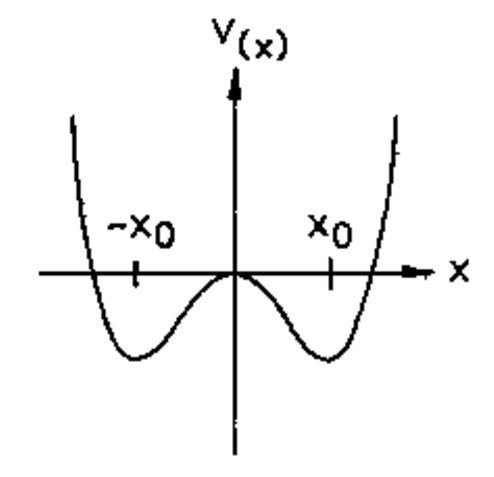
\includegraphics[]{figures/MexicoHutpotential.pdf}
    \caption{Darstellung des Mexico-Hut-Potentials in zwei Dimensionen. Zu erkennen sind die zwei möglichen Grundzustände $x = \pm x_0$ \cite{kleingrot}.}
    \label{fig:mexicohutpot}
\end{figure}
Anschaulich stellen wir uns vor, dass wir uns zunächst im Zentrum des Potentials befinden.
Das Potential besitzt eine globale Symmetrie, egal in welche Richtung wir schauen.
Das System wählt nun einen der beiden Grundzustände aus.
Für das gewählte Vakuum besteht jetzt allerdings die genannte Symmetrie nicht länger, da sich die Position des Grundzustandes bei Rotation des Potentials ändert.


\section{Ursprung der Neutrinomasse} %\cite{kleingrot}
\label{sec:neutrinomasse}

Als nur schwach wechselwirkende Teilchen ist zum jetzigen Zeitpunkt nur die Existenz linkshändiger Neutrinos $\nu_L$ und rechtshändiger Antineutrinos $\bar{\nu}_R$ nachgewiesen.
Diese sind über die Ladungs- und Paritätskonjugation $C P$ durch 
\begin{equation}
    (\nu_L)^{C P} = \bar{\nu}_R
    \label{eq:cpkonju}
\end{equation}
miteinander verknüpft.
Der Paritätsoperator $P$ transformiert dabei linkshändige in rechtshändige Teilchen und umgekehrt, die Ladungskonjugation überführt Teilchen in ihre Antiteilchen, ohne dabei ihre Händigkeit zu verändern.
Sind die ladungskonjugierten Teilchen zu $\nu_L$ bzw. $\bar{\nu}_R$ bisher nicht beobachtete, unabhängige Teilchen, sprechen wir von einem Dirac-Neutrino.
Ist $\nu_L$ bzw. $\bar{\nu}_R$ sein eigenes ladungskonjugiertes Teilchen, gilt
\begin{align*}
    (\nu_L)^C = \nu_L \,, && (\bar{\nu}_R)^C = \bar{\nu}_R \,.
\end{align*}
Die, nach dem italienischen Physiker Ettore Majorana benannten Majorana-Neutrinos lösen nach wie vor die Diracgleichung \eqref{eq:dirac}, es existieren allerdings nur zwei physikalisch unterscheidbare Zustände.
Diese beiden Majorana-Masseneigenzustände
\begin{align*}
    \nu_1 = \nu_L + \nu^{C P}_R \\
    \nu_2 = \nu_R + \nu^{C P}_L
\end{align*}
sind ihre eigenen Antiteilchen und bilden gemeinsam den Massenterm der Lagrangedichte $\mathcal{L}_M$, wie in \cite{kleingrot} dargestellt, durch
\begin{equation}
    \mathcal{L}_M = \mathcal{L}^L_M + \mathcal{L}^R_M = -\frac{1}{2} m^M_L \bar{\nu}_1 \nu_1 - \frac{1}{2} m^M_R \bar{\nu}_2 \nu_2 \,.
    \label{eq:lagrangedichtemajo}
\end{equation}
Dabei stellen $m^M_L$ bzw. $m^M_R$ als Massen die Kopplungsstärken zwischen $\nu_L$ und $\bar{\nu}_R$ bzw. $\nu_R$ und $\bar{\nu}_L$ dar.

Im Standardmodell lassen sich jedem Lepton die Leptonenzahl $+1$ und jedem Antilepton die Leptonenzahl $-1$ zuordnen. 
Über das Standardmodell hinaus wird die Leptonenzahl zur Beschreibung der Leptonenzahlsymmetrie oft über den sogenannten Leptonenzahloperator $L$ zugewiesen.
So erhalten auch Neutrinos als Leptonen eine Leptonenzahl.
Sind jedoch, wie oben beschrieben, Neutrinos und Antineutrino als Majoranateilchen identisch, ergibt die Zuordnung einer Leptonenzahl keinen Sinn mehr.
Die globale Leptonenzahlsymmetrie ist also, wenn auch nur sehr geringfügig, spontan gebrochen.

Zu den Mechanismen, die die Neutrinomasse als Majoranamasse annehmen, gehört beispielsweise der von Minkowski vorgeschlagene Seesaw-Mechanismus (engl. für Wippe), der die Kleinheit der Neutrinomassen durch das
Einführen eines zweiten, vergleichsweise sehr schweren Neutrinos, erklärt.
Die schweren Neutrinozustände stellen dabei die bisher nicht beobachtbaren Zustände des rechtshändigen Neutrinos, das, da es an keiner der bekannten Wechselwirkungen teilnimmt, auch steriles Neutrino genannt wird,
und das linkshändige Antineutrino, das gleichermaßen steril ist.
Die uns bekannten leichten Neutrinos wäre dann durch einen beinahe reinen Majoronamassenzustand beschreibbar \cite[Kap. 1.6.5]{kleingrot}.












\chapter{Neutrinos und Neutrinomischung in verschiedenen Basen}
\label{chap:neutrinobasen}

\section{Flavourbasis} %\cite[Kap. 2.1]{oberauer}
\label{subsec:flavourbasis}
Voraussetzung für die Neutrinooszillationen ist, dass Masseneigenzustände $\nu_i$ als Lösungen der Diracgleichung mit den Masseneigenwerten $m_i \neq 0 (i = 1, 2, 3)$ existieren.
Diese Masseneigenzustände bestimmen die Propagation des Neutrinos im Vakuum und müssen nicht zwangsläufig identisch zu den Flavoureigenzuständen sein.
Hier betrachten wir die Flavoureigenzustände $\nu_\alpha (\alpha = e, \mu, \tau)$ als Superposition der Masseneigenzustände mit
\begin{equation}
    \nu_\alpha = \sum_i U_{\alpha i} \nu^{(h_i)}_i \,,
    \label{eq:flavourbasis}
\end{equation}
wobei $U_{\alpha i}$ die unitäre Mischungsmatrix zwischen Massenbasis und Flavourbasis darstellt \cite[Kap. 2.1]{oberauer}.
Das Superskript $(h_i) = \pm 1$ beschreibt dabei die Helizität des Eigenzustands.


\section{Supernovae}

Im Inneren eines Sterns, der massiver als zehn unserer Sonnenmassen ist und sich dem Ende seines Lebens zuneigt, sind die Elemente nach absteigender Masse geschichtet.
Der Kern des Sterns, bestehend aus Eisen, Elektronen, Positronen, Photonen und vereinzelten Nukleonen, ist umgeben von Schichten aus Silizium, Sauerstoff, Kohlenstoff, Helium und Wasserstoff.
Je mehr Eisen der Stern fusioniert, desto weniger Material bleibt ihm zur weiteren Kernfusion übrig.
Zu diesem Zeitpunkt des Lebens des Sterns wird das Gleichgewicht zum nach innen wirkenden Gravitationsdruck durch den Strahlungsdruck der Elektronen nach außen aufrechterhalten. 
Auf Dauer ist dieses Gleichgewicht nicht stabil.

Die Elektronen und Protonen im Kern des Stern kombinieren im Prozess des Elektroneneinfangs zu einem Neutron und einem Elektronneutrino $e^- + p \rightarrow n + \nu_e$ \cite{supernovaepaper}.
So sinkt der Elektronendruck immer weiter, bis der Kern instabil wird und in sich zusammenstürzt, er kollabiert.
Die Kollapsgeschwindigkeit übersteigt dabei die Schallgeschwindigkeit im stellaren Medium, es erreicht also keine Information des zusammenbrechenden inneren Kerns den nachstürzenden äußeren Kern.
Mit einer anfänglichen Dichte von $10^9$ bis $10^{10} \, \si{\gram \per \centi\cubic\meter}$ erreicht er schnell Dichten, die in Atomkernen typisch sind.
In Zuge dessen ändert sich die Zusammensetzung im Kern.
Nun besteht er nur noch aus Protonen und Neutronen, die als Fermionen nach dem Pauliverbot niemals im exakt gleichen Zustand existieren dürfen.
Zusätzlich zu diesem Verbot kommt hinzu, dass Protonen sich auch aufgrund ihrer gleichen Ladung abstoßen.

Je dichter der Kern beim Kollaps also wird, desto drastischer erhöht sich der Druck nach außen, bis der Innendruck den Außendruck übersteigt und der Kern im \textit{Rebound} eine Schockwelle erzeugt, die nach außen durch den Stern propagiert.
Dabei verliert die Schockwelle durch das Aufbrechen des einfallenden Sternmaterials Energie.
Zusammen mit der Energie, die an Elektronneutrinos, die beim Elektroneneinfang mit den im Kern freiwerdenden Protonen entstehen, verloren geht, wird die Schockwelle im Kern verzögert, bevor sie vollends nach außen propagiert.
Der Kern des sterbenden Sterns mit seinem vergleichsweise kühlen Inneren und heißen, Neutrinos aller Flavours abstrahlenden Mantel wird nun als Protoneutronenstern bezeichnet.
Die im (auch Neutrinosphäre genannten) Mantel freiwerdenden Neutrinos entstehen in so großer Zahl, dass eine Leistung von mehr als $10^{45} \,\si{\watt}$ \cite{supernovaepaper} frei wird, die die verzögerte Schockwelle wiederbelebt.
So explodiert der Stern in einer spektakulären Explosion, die wir als Supernova bezeichnen.

\section{Materiebasis} %\cite{päspaper}
\label{subsec:materiebasis}

Dabei wird ein großer Teil der Supernovaenergie durch Neutrinos transportiert.
Ist es diesen nun möglich, bei der Propagation durch das Supernovamedium über den Zerfall $\tilde{\nu}^{(h_i)}_i (p_i) \rightarrow \tilde{\nu}^{(h_j)}_j (p_j) + J(q)$
Energie in Form von Majoronen $J$ mit Impuls $q$ abzustrahlen, kann sich, je nach Kopplungsstärke zwischen Neutrino und Majoron, das Energiespektrum der Supernova verändern.
Diese Zerfälle wirken sich auf das Oszillations- und Propagationsverhalten der Neutrinos aus und können mithilfe der Materiebasis beschrieben werden.

Drücken wir dabei das linkshändige vierkomponentige Feld $\nu_L$ in chiraler Darstellung der Gammamatrizen über ein zweikomponentiges Feld $\phi$ mit $\nu^T_L = (\phi, 0)^T$ aus, 
näheres dazu findet sich in \cite{komponentendinger}, lässt sich der Lagrangian in der Materiebasis als
\begin{equation}
    \mathcal{L}_\text{tot} = \mathcal{L}_0 + \mathcal{L}_\text{med} + \mathcal{L}_\text{int}
    \label{eq:materielagrange}
\end{equation}
mit
\begin{align*}
    \mathcal{L}_0          &=   i \sum_i \left[\phi^\dagger_i \left(\partial_t - \vec{\sigma} \times \nabla \right) \phi_i - \frac{m_i}{2} \left(\phi^T_i \sigma_2 \phi - \phi^\dagger_i \sigma_2 \phi^*_i\right) \right] \,,\\
    \mathcal{L}_\text{med} &= - \sum_{i j} \phi^\dagger_i V_{i j} \phi_j  \,,\\
    \mathcal{L}_\text{int} &= - J \sum_{i j} g^M_{i j} \left( \phi^T_i \sigma_2 \phi_j + \phi^\dagger_i \sigma_2 \phi^*_j \right)
\end{align*}
schreiben \cite{päspaper}.
Dabei beschreibt der freie Lagrangian $\mathcal{L}_0$ die Propagation im Vakuum, $\mathcal{L}_\text{med}$ die in der Potentialmatrix $V$ berücksichtigten Effekte von Materie und $\mathcal{L}_\text{int}$ Wechselwirkungen zwischen Neutrinos und Majoronen.
Die Kopplungsstärke zwischen Majoronen und Neutrinos der Massenbasis ist dabei in $g^M_{i j}$ zusammengefasst, $\vec{\sigma} = (\sigma_1, \sigma_2, \sigma_3)$ bezeichnet den Vektor der in \eqref{eq:paulimatrizen} zu findenden Paulimatrizen
und $m_i$ den Masseneigenwert des jeweiligen Neutrinos in der Massenbasis.
Wir berücksichtigen hier nur die einfachste Art der Majoronmodelle, also nehmen wir eine Proportionalität zwischen Kopplungs- und Massenmatrix $g^M_{i j} \propto m_{i j}$ an \cite{päspaper}.

Für gewöhnlich würden wir hier, um die Eigenzustände des bereits erwähnten Zerfalls $\tilde{\nu}^{(h_i)}_i (p_i) \rightarrow \tilde{\nu}^{(h_j)}_j (p_j) + J(q)$ zu bestimmen, 
die aus $\mathcal{L}_\text{tot}$ resultierenden Feldgleichungen 
\begin{equation}
    i \left(\partial_t - \vec{\sigma} \times \nabla \right) \phi_i + i m_i \sigma_2 \phi^*_i - \sum^3_j V_{i j} \phi_j = 0 \,,
\end{equation}
wie in \cite{komponentendinger} gezeigt, mithilfe von Planarwellenspinoren definiter Helizität lösen. 
Allerdings stimmen die so erhaltenden Lösungen mit den aus der Diagonalisierung der Mikheyev-Smirnov-Wolfenstein-Gleichung folgenden Lösungen überein.
Sie beschreibt die Zeitentwicklung schwacher Eigenzustände und die Mischung zwischen diesen und den Energieeeigenzuständen durch
\begin{equation}
    i \partial_t \nu^{(h)}_i = \left(H^\text{rel}_{i j} + U_{i \alpha} V_{\alpha \beta} U^\dagger_{\beta j}\right) \nu^{(h)}_j \,.
    \label{eq:MSW-gleichung}
\end{equation}
Aufgrund der geringen Massen und hohen Energien der Neutrinos, bei denen auch Energie- und Materieeigenzustände übereinstimmen, 
betrachten wir den hochrelativistischen Limes des Hamiltonians $H^\text{rel}_{i j} \approx \left(p + \frac{m^2_i}{2 p}\right) \delta_{ij}$ mit dem Kroneckerdelta
\begin{equation}
    \delta_{ij} = \begin{cases}
                    1, \quad i=j \\
                    0, \quad \text{sonst} \,.
                  \end{cases}
                  \label{eq:kronecker}
\end{equation}
Dabei ist $V$ die diagonale Potentialmatrix der schwachen Basis, also
\begin{equation}
    V = \left( \begin{array}{c c c}
        V_C + V_N   &   0     &     0   \\ 
        0           &   V_N   &     0   \\ 
        0           &   0     &     V_N  \\
        \end{array}\right) \,,
\end{equation}
wobei $V_C = \sqrt{2} h G_F n_B (Y_\text{e}) + Y_{\nu_\text{e}}$ das von geladenen Strömen erzeugte Potential und 
$V_N = \sqrt{2} h G_F n_B \left(-\frac{1}{2} Y_N + Y_{\nu_\text{e}}\right)$ das durch ungeladene Ströme erzeugte Potential beschreiben.
Mit der Baryonendichte $n_B$ des betrachteten Mediums gilt für ein beliebiges Teilchen $i$ mit korrespondierendem Antiteilchen $\bar{i}$ $Y_i = \frac{n_i - n_{\bar{i}}}{n_B}$ \cite{päspaper}.
Geladene Ströme bezeichnen dabei schwache Wechselwirkungen, bei denen ein $W^+$- oder $W^-$- Boson ausgetauscht wird und ungeladene Ströme nur unter Austausch von neutralen $Z$-Bosonen stattfindende schwache Wechselwirkungen.

Aus der Diagonalisierung der rechten Seite der MSW-Gleichung \cite{komponentendinger, PhysRevD.37.1935} folgen die Materieeigenzustände
\begin{equation}
    \tilde{\nu}^{(h_i)}_i = \sum_i \tilde{U}_{i j} \nu^{(h_j)}_j \,.
    \label{eq:materiebasis}
\end{equation} 
Ähnlich wie die Flavoureigenzustände lassen sie sich als Superposition der Masseneigenzustände beschreiben.
Sie unterscheiden sich lediglich in der Mischungsmatrix $\tilde{U}$.

Hier können wir die in \autoref{subsec:flavourbasis} auftretende Mischungsmatrix $U$ als
\begin{equation}
    U = U_{2 3} \, U_{1 3} \, U_{1 2} \, U_0
    \label{eq:kopplungflavour}
\end{equation}
parametrisieren.
Bei den Matrizen $U_{i j}$ handelt es sich dabei um Rotationsmatrizen, die in der $i j$-Ebene eine Rotation um den Winkel $\theta_{i j}$ durchführen.
Die in \autoref{sec:neutrinomasse} behandelte mögliche CP-Verletzung findet sich als Phase in der Matrix $U_0$ mit $U_0 = \text{diag}(1, \mathrm{e}^{-2 i \delta_1}, \mathrm{e}^{-2 i \delta_2})$ wieder, wobei
$\delta_1$ und $\delta_2$ komplexe, beliebige Majoranaphasen darstellen\cite{neutrinorotmat}.

Wie im Chooz-Experiment festgestellt wurde, ist der Chooz-Winkel $\theta_{1 3}$ nicht, wie lange Zeit angenommen, null \cite{theta13}.
Nach aktuellen Daten der Particle Data Group gilt $\sin^2 \left(\theta_{1 3} \right) = \num{2.20 +- 0.07} \cdot 10^{-2}$ \cite{neutrinospdg}.

Wir können $\theta_{1 2}$ als solaren Mischungswinkel $\theta_\odot$ und $\theta_{2 3}$ als atmosphärischen Mischungswinkel $\theta_\text{atm}$ identifizieren.
Da zusätzlich, vor allem für leichte Neutrinos in der Nähe der Neutrinosphäre der Supernova, $|V_{\alpha \alpha}| \gg \frac{m^2_i}{2 p}$ für alle Elemente der Potentialmatrix gilt, unterscheiden sich die Materieeigenzustände nur um eine
beliebige Drehung $\theta'$ in der $\nu_\mu$ - $\nu_\tau$ Ebene von den Eigenzuständen der schwachen Basis.
Wir wählen $\theta' = -\theta_{2 3}$, um möglichst einfache Ausdrücke der Materieeigenzustände zu erhalten, wie sie in \autoref{tab:materieeigis} dargestellt sind.
\begin{table}[H]
    \centering
    \begin{tabular}{S S S}
      \toprule
    {Materieeigenzustände $\tilde{\nu}^{(h_i)}_i$} & {Schwache Eigenzustände $\nu_{\alpha'}$} & {Potential $V$} \\
      \midrule
       {$\tilde{\nu}^+_1$} & {$\bar{\nu}_e$}                                                        &  {$- (V_C + V_N)$} \\
       {$\tilde{\nu}^+_2$} & {$\bar{\nu}_{\mu'}  = c_{2 3} \bar{\nu}_\mu - s_{2 3} \bar{\nu}_\tau$} &  {$- V_N$} \\
       {$\tilde{\nu}^+_3$} & {$\bar{\nu}_{\tau'} = s_{2 3} \bar{\nu}_\mu + c_{2 3} \bar{\nu}_\tau$} &  {$- V_N$} \\
       {$\tilde{\nu}^-_1$} & {$\nu_{\mu'}        = c_{2 3} \nu_\mu       - s_{2 3} \nu_\tau$}       &  {$V_N$} \\
       {$\tilde{\nu}^-_2$} & {$\nu_{\tau'}       = s_{2 3} \nu_\mu       + c_{2 3} \nu_\tau$}       &  {$V_N$} \\
       {$\tilde{\nu}^-_3$} & {$\nu_e$}                                                              &  {$V_C + V_N$} \\
    \bottomrule
    \end{tabular}
    \caption{Materieeigenzustände $\tilde{\nu}^\pm_i$ positiver und negativer Helizität im Limes $|V_{\alpha \alpha}| \gg \frac{m^2_i}{2 p}$ als Rotation der schwachen Eigenzustände. Die Eigenzustände sind dabei so
            angeordnet, dass das Potential in der Tabelle nach unten hin ansteigt. Es gilt $c_{2 3} = \cos(\theta_{2 3})$ und $s_{2 3} = \sin(\theta_{2 3})$.}
    \label{tab:materieeigis}
\end{table}

Genauso lassen sich auch die Kopplungsmatrixelemente $\tilde{g}_{i j}$ der Materiebasis als Rotation der Elemente der schwachen Basis identifizieren.
In den hier betrachteten Modellen ist die Kopplungsmatrix der Massenbasis diagonal, es gilt
\begin{equation}
    g^W = \left( \begin{array}{c c c}
        g_1         &   0     &     0   \\ 
        0           &   g_2   &     0   \\ 
        0           &   0     &     g_3  \\
    \end{array}\right) \,.
    \label{eq:schwachekopplung}
\end{equation}
Damit ist
\begin{equation}
    g_{\alpha' \beta'} \equiv \ \tilde{g}_{i j} = U(-\theta_{2 3}) \, g^W_{\alpha \beta} \, U^T(-\theta_{2 3}) = U_{1 3} U_{1 2} \, U^*_0 \, g^M_{i j} \, U^\dagger_0 \, U_{1 2} U_{1 3} \,,
\end{equation}
wenn wir zusätzlich benutzen, dass die schwache Kopplungsmatrix und die der Massenbasis über $g^W = U \, g^M \, U^T$ verknüpft sind.
Die Matrixelemente $|g_{ij}|$ bezeichnen wir wie folgt:
\begin{align}
    \tilde{g} &= \left( \begin{array}{c c c}
        g_{ee}                  &   g_{e \mu'}          &     g_{e \tau'}       \\ 
        g_{e \mu'}              &   g_{\mu' \mu'}       &     g_{\tau' \mu'}    \\ 
        g_{e \tau'}             &   g_{\tau' \mu'}      &     g_{\tau \tau}     \\
    \end{array}\right) \label{eq:materiekoppmat} \,.
\end{align}

Die Kopplungsparameter $g_2$ und $g_3$ lassen sich dabei in Abhängigkeit von $g_1$ und $m_1$, also der Masse des ersten Masseneigenzustands, ausdrücken als
\begin{align}
    g_2 = g_1 \sqrt{1 + \frac{\Delta m^2_\odot}{m^2_1}}\,, && g_3 = g_1 \sqrt{1 + \frac{\Delta m^2_\odot + \Delta m^2_\text{atm}}{m^2_1}} \,,
    \label{eq:g2g3}
\end{align}
wobei wir die Definitionen $\Delta m^2_{1 2} = m^2_2 - m^2_1 = \Delta m^2_\odot$ und $\Delta m^2_{23} = m^2_3 - m^2_2 = \Delta m^2_\text{atm}$ benutzen.
So ist ein Zusammenhang der Kopplungsmatrizen aller drei Basen hergestellt, den wir verwenden, um die Einschränkungen auf die Kopplungsstärken deutlich zu machen.


%% Unnötige Kopplungsmatrix
%    &= \left( \begin{array}{c c c}
%        c^2_{1 2} c^2_{1 3} g_1 + s^2_{12} c^2_{13} \mathrm{e}^{-2 i \delta_1} g_2 + s^2_{13} \mathrm{e}^{-2 i \delta_2}  g_3               &   -s_{12}c_{12}c_{13} g_1 + c_{12} s_{12} c_{13} \mathrm{e}^{-2 i \delta_1} g_2       &   -c^2_{12} s_{13} c_{13} g_1 + s^2_{12} c^2_{13} \mathrm{e}^{-2 i \delta_1} g_2 + s_{13} c_{13} \mathrm{e}^{-2 i \delta_2} g_3  \\ 
%        -s_{12}c_{12}c_{13} g_1 + c_{12} s_{12} c_{13} \mathrm{e}^{-2 i \delta_1} g_2                                                       &   s^2_{12} g_1 + c^2_{12} \mathrm{e}^{-2 i \delta_1} g_2                              &   s_{12} c_{12} s_{13} g_1 + s_{12}c_{12}s_{13} \mathrm{e}^{-2 i \delta_1} g_2   \\ 
%        -c^2_{12} s_{13} c_{13} g_1 + s^2_{12} c^2_{13} \mathrm{e}^{-2 i \delta_1} g_2 + s_{13} c_{13} \mathrm{e}^{-2 i \delta_2} g_3       &   s_{12} c_{12} s_{13} g_1 + s_{12}c_{12}s_{13} \mathrm{e}^{-2 i \delta_1} g_2        &   c^2_{21} s^2_{13} g_1 + s^2_{12}s^2_{13} \mathrm{e}^{-2 i \delta_1} g_2 + c^2_{13} \mathrm{e}^{-2 i \delta_2} g_3  \\
%    \end{array}\right)





\chapter{Ausschlussregionen der Kopplungsparameter}


Mit den bisher zusammengestellten Einschränkungen auf $g_i$ und $m_1$ ist es uns, gemeinsam mit der Ausschlussregion auf $|g_{i j}|$ möglich, Grafiken zu erstellen, die uns die zulässigen Bereiche für $g_1$ und $m_1$ deutlich machen.
Dazu betrachten wir die einzelnen Einträge in \eqref{eq:materiekoppmat} und nutzen die Ausdrücke in \eqref{eq:g2g3}, um $|g_{i j}|$ nur in Abhängigkeit von $g_1$ und $m_1$ zu schreiben.
Somit ist es uns möglich, anschließend wahlweise $g_1$ in Abhängigkeit von $m_1$ oder $m_1$ in Abhängigkeit von $g_1$ auszudrücken.
Hier entscheiden wir uns für $m_1 (g_1)$, um einen besseren Vergleich zu \cite{päspaper} herstellen zu können.
Für alle folgenden Plots werden die LMA-MSW-Werte
\begin{align*}
    \sin^2\theta_\odot = \num{0.307}\,, && \Delta m^2_\odot = \num{7.53} \cdot 10^{-5} \si{eV}^2\,, && \Delta m^2_\text{atm} = \num{2.453} \cdot 10^{-3} \si{\eV}^2
\end{align*}
verwendet \cite{neutrinospdg}.

\section{Ausschlussregion für $g_{ee}$}

Beginnen wir zunächst mit der Kopplung $g_{ee}$.
Hier gehen wir die Rechnung einmal Schritt für Schritt durch, da die Rechenschritte allerdings nur aus Umformungen und trivialen Operationen besteht und für alle Kopplungen dem gleichen Schema folgt, werden wir auf die Berechnungen der anderen
Kopplungen nicht näher eingehen.

Wie in \eqref{eq:materiekoppmat} zu erkennen ist, gilt
\begin{equation}
    g_{ee} = g_1 \cos^2 \theta_\odot + g_2 sin^2 \theta_\odot \mathrm{e}^{-2 i \delta} \,.
    \label{eq:g_ee}
\end{equation}
Unter der Nutzung von
\begin{equation*}
    g_2 = g_1 \sqrt{1 + \frac{\Delta m^2_\odot}{m^2_1}}
\end{equation*}
aus \eqref{eq:g2g3} erhalten wir
\begin{equation*}
    g_1 \sqrt{1 + \frac{\Delta m^2_\odot}{m^2_1}} = \frac{g_{ee} - g_1 \cos^2 \theta_\odot}{sin^2 \theta_\odot} \mathrm{e}^{2 i \delta} \,.
\end{equation*}
Dividieren wir durch $g_1$, quadrieren die gesamte Gleichung und bringen die $1$ auf die andere Seite, erhalten wir
\begin{equation*}
    \frac{\Delta m^2_\odot}{m^2_1} = \left(\frac{g_{ee} -  \cos^2 \theta_\odot \, g_1}{sin^2 \theta_\odot \, g_1} \mathrm{e}^{2 i \delta} \right)^2 - 1 \,.
\end{equation*}
Jetzt müssen wir nur noch den Kehrwert bilden und die Wurzel ziehen
Dann ist durch die Wurzel der Gleichung das Ergebnis
\begin{equation}
    m_1 = \sqrt{\frac{\Delta m^2_\odot}{\left(\frac{g_{ee} -  \cos^2 \theta_\odot \, g_1}{sin^2 \theta_\odot \, g_1} \mathrm{e}^{2 i \delta} \right)^2 - 1}}
    \label{eq:m_1g_ee}
\end{equation}
gegeben.

Da die CP-verletzende Phase $\delta$ frei wählbar ist, wählen wir hier zur Darstellung der Kopplung stets die beiden Extreme $\delta = 0$, also einen maximal positiven, und $\delta = \frac{pi}{2}$, also einen maximal negativen Phasenbeitrag.
An \eqref{eq:m_1g_ee} wird aber schnell erkennbar, dass genau diese Wahl der Phasen keinerlei Auswirkungen auf die Parametrisierung von $m_1$ zu haben scheint.
Denn mit $\mathrm{e}^{2 i \frac{\pi}{2}} = -1$ wird das negative Vorzeichen durch das Quadrat wieder aufgehoben.
Wir sehen aber, dass die gewählte Phase zumindest für die Bestimmung des durch die in \autoref{subsec:KATRIN} erläuterte Massengrenze auftretenden Cutoff nicht ganz irrelevant ist.

Um genau diesen Cutoff an der Massengrenze zu ermitteln, stellen wir \eqref{eq:g_ee} außerdem nach $g_1$ statt $m_1$ um, erhalten
\begin{equation}
    g_1 = \frac{g_{ee}}{\cos^2\theta_\odot + \sqrt{1 + \frac{\Delta m^2_\odot}{m^2_1}} \sin^2\theta_\odot \mathrm{e}^{-2 i \delta}} 
    \label{eq:g1cutoffg_ee}
\end{equation}
und setzen für $m_1$ schließlich das gewünschte Limit ein.
Wählen wir $m_1 \gg \Delta m^2_\odot$, beeinflusst die Wahl von $m_1$ nicht länger das Ergebnis von $g_1$ und es entsteht das in \autoref{fig:m_1g_ee} erkennbare divergente Verhalten.
Hier ist die Phasenabhängigkeit offensichtlich.
Wählen wir eine Phase von $\delta = \frac{\pi}{2}$ ist es möglich, dass sich die beiden Terme in \eqref{eq:g1cutoffg_ee} gegenseitig eliminieren.
So entstehen zwei Zweige, die an unterschiedlichen Stellen nahezu parallel zur $y$-Achse $m_1 = \SI{0.8}{\eV}$ erreichen.
Dazu sei gesagt, dass, da sie die Einschränkung von $|g_{i j}|$ nur auf den Betrag beziehen, immer vier Kurven, jeweils zwei für die positiven und zwei für die negativen Ober- und Untergrenzen entstehen.
\begin{figure}[H]
    \centering
    \includegraphics[width=\textwidth]{build/m1g1g_ee.pdf}
    \caption{Neutrinomasse $m_1$ in Abhängigkeit des Kopplungsparameters $g_1$ für $g_{ee}$. Die durchgezogenen blauen Linien stellen dabei die untere und obere Grenze $g_{ee} = 3 \cdot 10^{-7}$ bzw. $g_{ee} = 2 \cdot 10^{-5}$
            mit einer Phase von $\delta = 0$, die gestrichelten Linien die Grenzen bei einer Phase von $\delta = \frac{\pi}{2}$ dar. Gemeinsam mit den türkisen Linien der negativen Grenzen auf $|g_{ee}|$ entsteht so die blau
            gefüllte Ausschlussfläche. Die rote Fläche kennzeichnet dabei den durch KATRIN ausgeschlossen Massenbereich von $m_1 > \SI{0.8}{\eV}$.}
    \label{fig:m_1g_ee}
\end{figure}
Die Ausschlussregion ist dabei so gewählt, dass ein möglichst großer Parameterbereich übrig bleibt.
Hier werden also nur die innersten Kurven zur Bildung der Fläche verwendet.
Für einen bestimmten, relativ schmalen Wertebereich von $g_1$ wird in \eqref{eq:m_1g_ee} das quadrierte Argument im Nenner der Wurzel kleiner als 1.
Damit wird die Wurzel imaginär und es entsteht die beobachtbare Lücke im Plot.
Auffällig ist auch das asymptotische Verhalten der Äste für verhältnismäßig große $g_1$.
Wird $g_1$ groß gegen die gewählte Grenze von $g_{ee}$, gilt näherungsweise 
\begin{equation*}
    \frac{g_{ee} -  \cos^2 \theta_\odot \, g_1}{sin^2 \theta_\odot \, g_1} \mathrm{e}^{2 i \delta} \approx \frac{\cos^2 \theta_\odot \, g_1}{sin^2 \theta_\odot \, g_1} \mathrm{e}^{2 i \delta}
    = \frac{\cos^2 \theta_\odot}{sin^2 \theta_\odot} \mathrm{e}^{2 i \delta} \,.
\end{equation*}
In dem Fall ist $m_1$ also durch
\begin{equation*}
    m_1 = \sqrt{\frac{\Delta m^2_\odot}{ \left(\frac{\cos^2 \theta_\odot}{sin^2 \theta_\odot} \mathrm{e}^{2 i \delta}\right)^2 - 1}}
\end{equation*}
gegeben, $m_1$ ist also konstant. \\
Diese asymptotische Konvergenz gegen $m_1 \approx \num{7.9695} \cdot 10^{-4} \, \si{\eV}$ tritt für alle Werte von $g_{ee}$ früher oder später ein.



\appendix
% Hier beginnt der Anhang, nummeriert in lateinischen Buchstaben
\chapter{Anhang}

\backmatter
\printbibliography

\cleardoublepage
% From https://www.tu-dortmund.de/studierende/im-studium/pruefungsangelegenheiten/allgemeine-vordrucke/
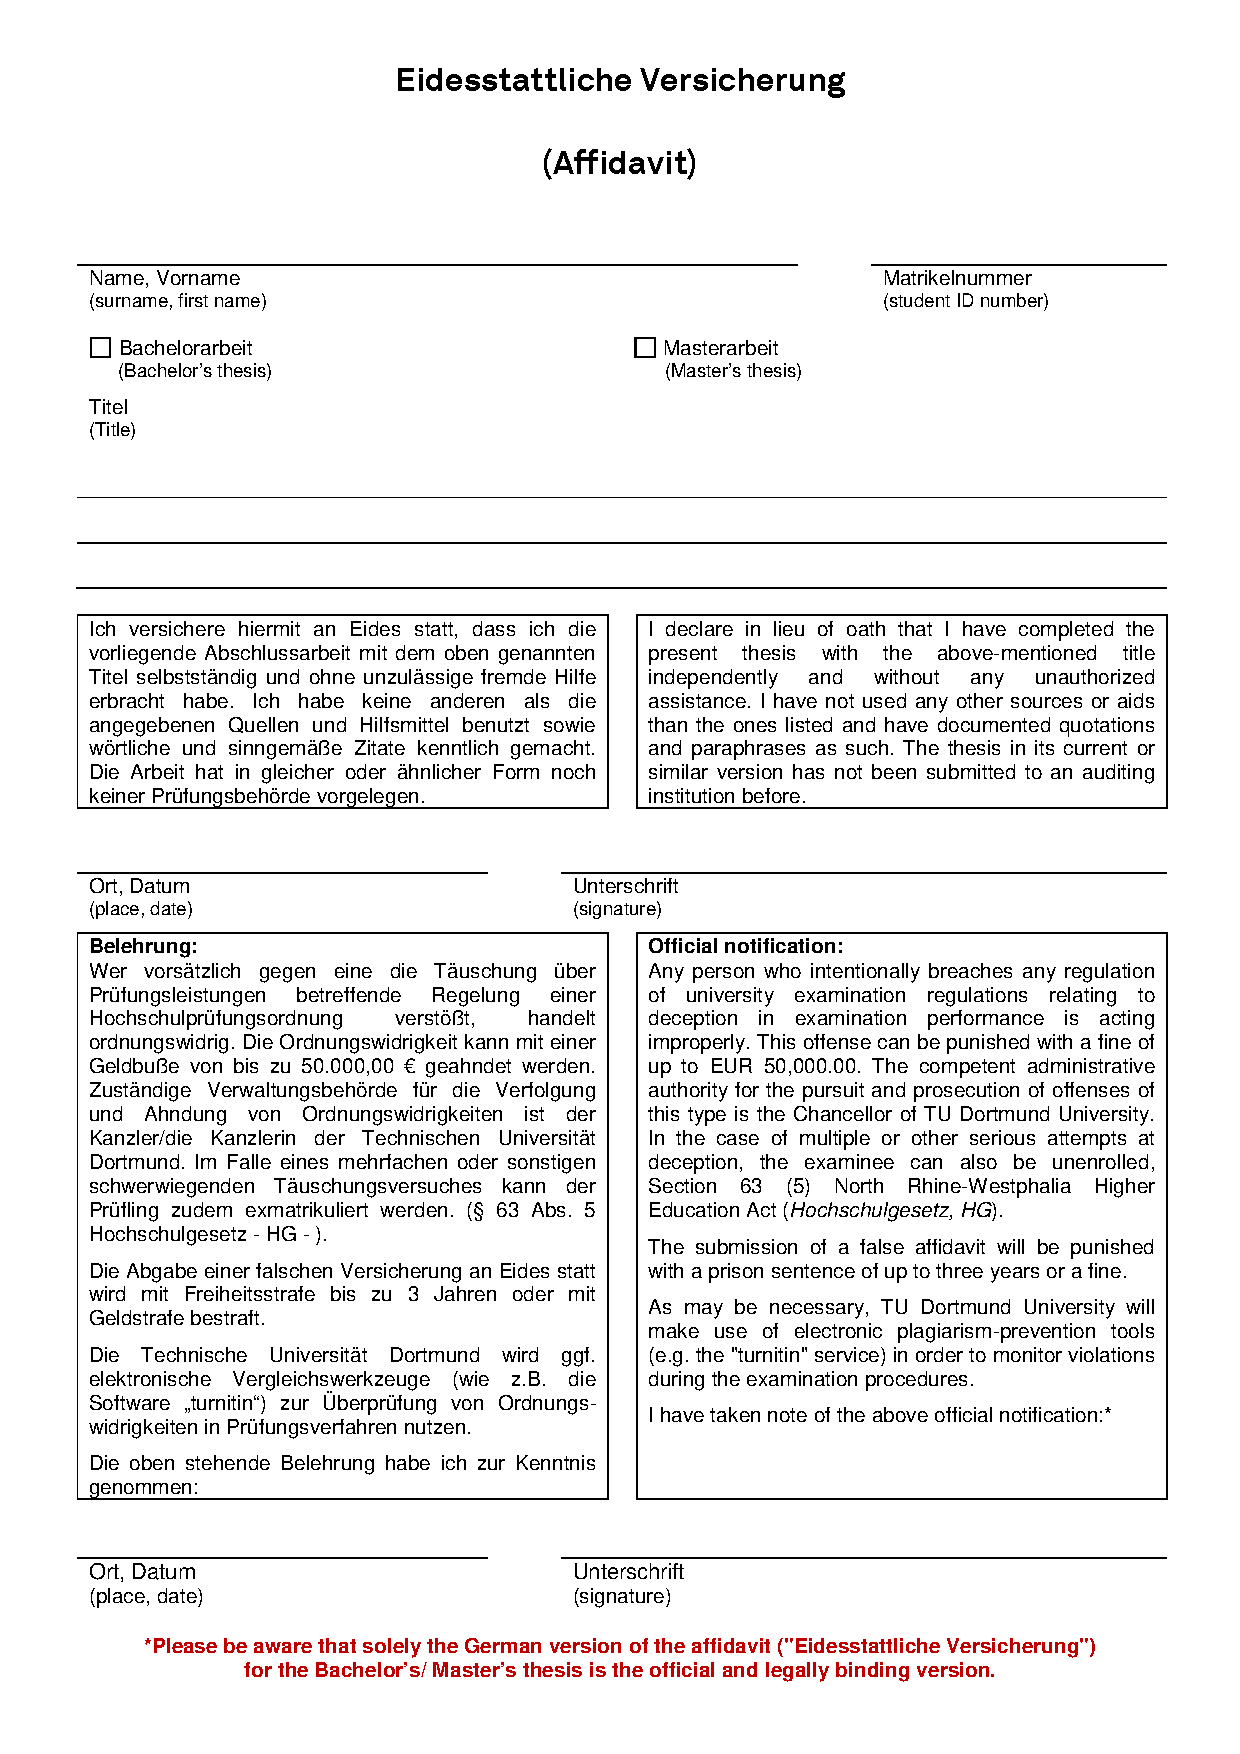
\includepdf{content/Eidesstattliche_Versicherung.pdf}

\end{document}
